\chapter{Propozycja rozwiązania}

\section{Tworzenie aplikacji od podstaw}
\label{nowa_aplikacja}
\subsection{Nowe podejście do architektury systemu}
\label{clean_architecture}
Największą przeszkodą w testowaniu aplikacji androidowych jest niestety sam Android. Im większy \textit{coupling} między warstwami, tym trudniej jest pisać testy jednostkowe. Rozważmy więc przekształcenie modelu aplikacji Android opisanego na początku poprzedniego rozdziału w następujący sposób:

\begin{figure}[!htb]
    \centering
    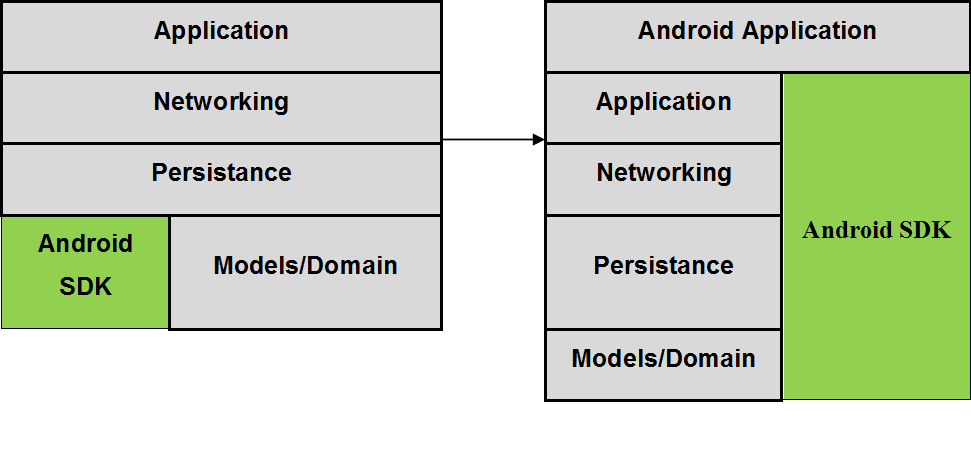
\includegraphics[width=13cm]{imgs/ch4_opis_rozwiazania_1.png}
    \caption
{Zmodyfikowana struktura aplikacji Android: Clean Architecture}
    \label{fig:opis_rozwiazania}
\end{figure} 

Nowy model aplikacji oddziela (przynajmniej w teorii) warstwy Application, Networking, Persistance oraz Model/Domain od środowiska Android SDK, a co za tym idzie nie musimy umieszczać odwołania do tego środowiska praktycznie w każdym pliku (wyrażenie \texttt{import android.*}). Dopiero najwyższą warstwą jest warstwa Aplikacja Android. W takim podejściu staramy się użyć Androida jako pewnego rodzaju \textit{pluginu} do naszej aplikacji i uniezależnić warstwę logiczną od reszty warstw. Czyli najpierw napiszemy aplikację, która będzie oddzielona od Android SDK (na przykład w czystej Javie), potem dołączymy do tego android SDK i złączymy to wszystko w Aplikację Android. W ten sposób zapewnimy, że kod, który stanowi podstawę naszej aplikacji, czyli jej logikę działania, był przetestowany tak jak należy, czyli w oddzieleniu od reszty warstw.

\subsection{Zastosowanie techniki \textit{Test Driven Development} przy tworzeniu oprogramowania}
Jak już autor wspomniał w rozdziale \ref{test_driven_development} dotyczącym metodologii TDD, wytwarzanie oprogramowania zaczynając od testowania powoduje, że zostanie napisanie tylko tyle aplikacji, ile to jest ujęte w wymaganiach. A co za tym idzie jej stopień komplikacji zostanie ograniczony do niezbędnego minimum. Zastosowanie tej techniki w przypadku aplikacji tworzonych pod Android z wykorzystaniem uporządkowanej architektury pozwoli na zwiększenie testowalności aplikacji. 

\begin{figure}[!htb]
    \centering
    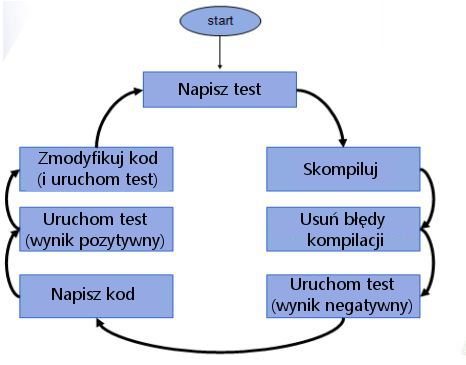
\includegraphics[width=10cm]{imgs/ch4_tdd.jpg}
    \caption
{Schemat kodowania w technice TDD}
    \label{fig:tdd_schema}
\end{figure} 

Korzyści, których można się spodziewać po zastosowaniu tej techniki są następujące:

\begin{itemize}
\item
Wczesne wykrywanie błedów. Odporność na błedy regresyjne. Programista poprawia swoje błędy na bieżąco.
\item
Łatwiejszy refaktoring kodu.
\item
Dobrze napisane testy stają się dokumentacją kodu.
\item
Lepiej zaprojektowane interfejsy. Technika projektowania testów za pomocą \textit{user stories} zmusza do lepszego przemyślenia rozwiązań i dokładnego określenia zadań. 
\item
Uproszczona integracja, łatwiejsze łączenie różnych fragmentów kodu poddanych wcześniej testom. Mniej błedów przedostaje się do etapu testów systemowych.
\item
Automatyzacja i powtarzalność \textit{(contignous integration)}: testy można uruchamiać regularnie o określonych porach lub na pewnych etapach produkcji. 
\item
Możliwość przetestowania funkcjonalności bez uruchamiania oprogramowania.
\end{itemize}

Wady \textit{Test Driven Development} dotyczą głównie wykorzystania czasu w projekcie. Wymagany jest:

\begin{itemize}
\item
Dodatkowy czas na stworzenie testów jednostkowych - deweloper potrzebuje czasem nawet o 40 procent więcej czasu na wykonanie tych samych zadań.
\item
Dodatkowy czas na utrzymanie testów - przy wprowadzaniu zmian w istniejącej funkcjonalności należy pamiętać, że potrzebny jest również czas na modyfikację istniejących testów jednostkowych.
\end{itemize}

\subsection{Automatyzacja testów jednostkowych}
Testy automatyczne powinny przyczyniać się do poprawy jakości dostarczając szybkiej - dużo szybszej niż w przypadku testowania manualnego - informacji zwrotnej na temat działania programu. Dodatkowo, szybka informacja zwrotna jest potwierdzeniem, że programista niczego nie uszkodził podczas modyfikowania gotowych funkcji.
Automatyzacja testów nie ma sensu, jeżeli jej koszt jest większy niż korzyści, które przynosi. Z analizy rysunku \ref{fig:idealna_piramida} z rozdziału \ref{piramida?testowania} można wnioskować, że największą korzyść przynosi automatyzacja testów jednostkowych. Są relatywnie łatwe do napisania, wykonują się w ułamkach sekund i są równiez łatwe do modyfikacji. Unit testy są solidną podstawą automatycznych testów regresyjnych.

\subsection{Kod jako dokumentacja programu}


\section{Różne podejścia do uporządkowania architektury}
\subsection{Architektura cebulowa - \textit{The Onion Architecture}}
Jeffrey Pallermo w połowie 2008 roku opublikował na swoim blogu serię artykułów\cite{website:architect:onion}, w których zaproponował inne od klasycznego podejście do warstw w aplikacji. Zauważył, że uzależnienie warstwy biznesowej od warstwy danych niekorzystnie wpływa na stabilność warstwy biznesowej, która z założenia powinna być niezależna od wprowadzania nowych technologii do warstwy bazodanowej. Stare podejście tego nie zapewniało. W większości przypadków warstwa biznesowa musiała być modyfikowana, a przynajmniej rekompilowana podczas modyfikacji warstwy dostępu do danych.

W zaproponowanym przez Palermo modelu, im warstwy położone są w architekturze głębiej, tym mniej podatne są na zmiany. Zależności mogą być zwrócone tylko w jedną stronę - do wnętrza "cebuli". W ten sposób w centrum znajdzie się model domeny, a na zewnątrz - warstwa bazodanowa. Jest to podejście nazywane \textit{odwróceniem zależności\footnote{Dependency Inversion Principle (DIP) - zasada mówiąca, że moduły wysokopoziomowe nie powinny zależeć od modułów niskopoziomowych. Obie grupy powinny zależeć od abstrakcji. Abstrakcje natomiast nie powinny zależeć od szczegółowych rozwiązań, tylko odwrotnie.}} i wymaga od programistów zastosowania odpowiednich technik projektowych, między innymi \textit{wstrzykiwania zależności\footnote{Dependency Injection (DI) – wzorzec projektowy i wzorzec architektury oprogramowania polegający na usuwaniu bezpośrednich zależności pomiędzy komponentami na rzecz architektury typu plug-in. Źródło: Wikipedia}}.

Warstwy wewnętrzne definiują interfejsy, za pomocą których mogą komunikować się z warstwami zewnętrznymi. Dzięki temu programiści nie muszą implementować na przykład dostępu z warstwy biznesowej do bazy danych w warstwie danych, zaimplementują tylko odpowiedni interfejs.

\begin{figure}[!htb]
    \centering
    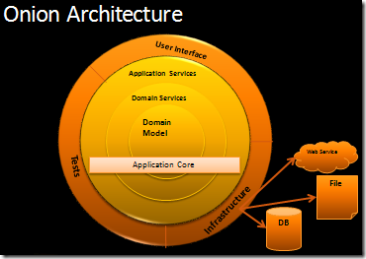
\includegraphics[width=10cm]{imgs/ch4_onion_architecture.png}
    \caption
{Onion architecture według Jeffrey'a Palermo. Źródło: \url{http://jeffreypalermo.com/blog/the-onion-architecture-part-1}}
    \label{fig:onion_architecture}
\end{figure} 

Kluczowe założenia architektury cebulowej:
\begin{itemize}
\item 
Aplikacja zbudowana jest według niezależnego modelu obiektowego.
\item
Warstwy wewnętrzne definiują interfejsy. Warstwy zewnętrzne te interfejsy implementują.
\item
Kierunek \textit{sprzężenia} jest od warstwy zewnętrznej do wewnętrznej.
\item
Cały kod rdzenia aplikacji (\textit{Object Model, Object services, Application Services}) może zostać skompilowany i wykonany bez kontaktu z infrastrukturą i interfejsem użytkownika.
\end{itemize}


\subsection{Architektura portów i adapterów - \textit{Ports and Adapters Architecture}}
Opracowana w 2005 roku przez Alistaira Cockburna\footnote{Alistair Cockburn - jeden z inicjatorów ruchu Agile. Jest współautorem wydanego w 2001 roku manifestu Agile. W roku 2005 pomagał współtworzyć deklarację 'PM Declaration of Interdependence'. Propagator przypadków użycia jako dokumentacji procesów biznesowych oraz wymagań co do zachowania oprogramowania. Źródło: Wikipedia} architektura niegdyś znana była pod nazwą architektury heksagonalnej.\cite{website:architect:hexagonal}. Nazwa "heksagonalna" przyjęła się, ponieważ kiedyś znane były tylko trzy porty wejściowe i trzy porty wyjściowe, stąd wszystkie schematy rysowane były jako foremny sześciokąt. Wraz ze wzrostem liczby portów wejściowych i wyjściowych zmieniono nazwę na \textit{Ports \& Adapters}, nie zmieniono natomiast zasady przedstawiania architektury na schematach, co przedstawia rysunek \ref{fig:hexagonal_architecture}.

\begin{figure}[!htb]
    \centering
    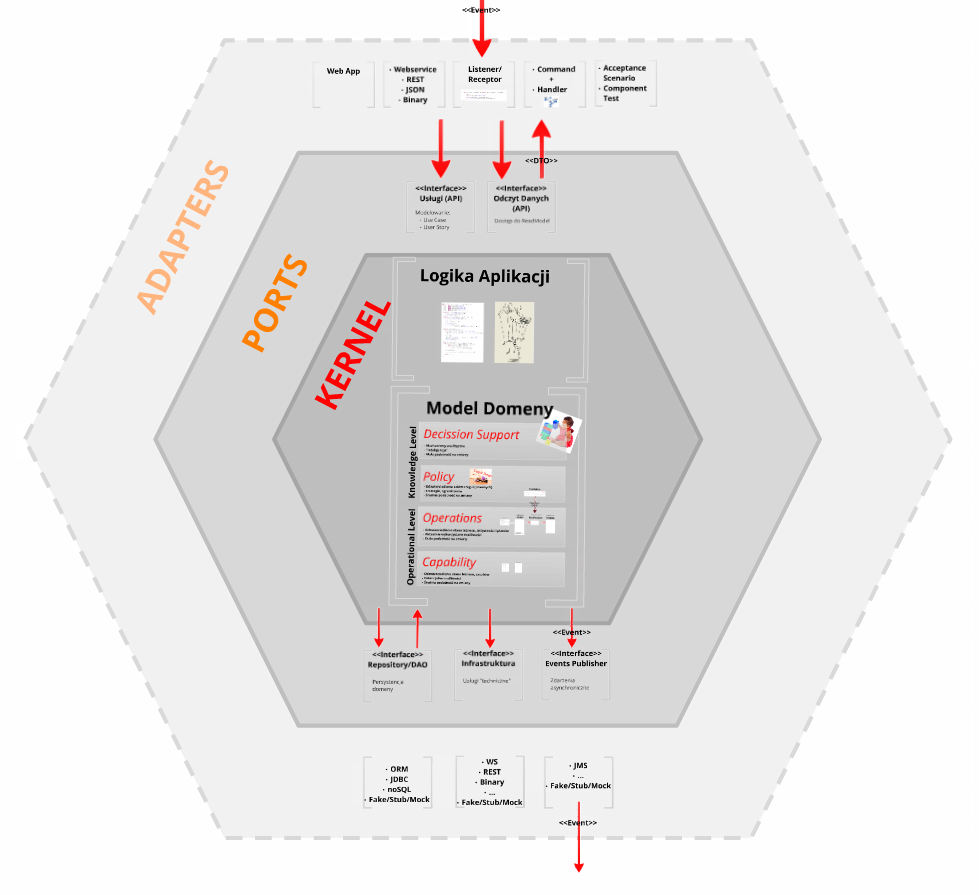
\includegraphics[width=13cm]{imgs/ch4_hexagonal_architecture_2.png}
    \caption
{Architektura heksagonalna. Opracowanie: Sławomir Sobótka. Źródło: \url{https://prezi.com/p0psif9qixgz/ports-adapters}}
    \label{fig:hexagonal_architecture}
\end{figure} 

Idea jest bardzo podobna do architektury cebulowej: w centrum znajduje się jądro aplikacji, czyli model domeny i logika biznesowa, odpowiedzialna za kluczowe działania programu. Jądro otoczone jest przez warstwę portów, zawierającą porty zarówno wejściowe, jak i wyjściowe. Zewnętrzną warstwą jest warstwa adapterów. W szczegółach przedstawia się to następująco:

\paragraph{Jądro - \textit{Kernel}}
Jądro oferuje model domeny i logikę biznesową: ogólne możliwości aplikacji, operacje, logikę operacji oraz mechanizmy wspierania decyzji, co już w wymienionej kolejności stanowi architekturę warstwową. Warstwa również może być podzielona na kilka poziomów logiki. 

\paragraph{Porty - \textit{Ports}}
Porty są to interfejsy usług: API, odczyt danych (wejściowe), oraz interfejsy repozytoriów czy DAO\footnote{Data Access Object – komponent dostarczający jednolity interfejs do komunikacji między aplikacją a źródłem danych.}, sterowniki do różnego rodzaju maszyn, urządzeń, odbiorników GPS czy radia (wyjściowe). Jądro za pomocą portów wyjściowych jest również w stanie emitować zdarzenia. Zdarzenia są techniką odwracania kontroli, czyli przyjęta jest znów zasada, że warstwa wewnętrzna nie chce mieć kontroli nad warstwą zewnętrzną. 

\paragraph{Adaptery - \textit{Adapters}}
Szczególnym adapterem jest aplikacja webowa. Może odbierać również zdarzenia od innych modułów systemowych, jeżeli architektura systemowa jest modułowa (Listener/Receptor zdarzeń). Adapter deleguje to zdarzenie do portów. Adapter powinien mieć najgłupszy jak to tylko możliwe. W ten sposób powstaje nam taki klaster heksagonalnych modułów.

Testy jednostkowe penetrują jądro, testy integracyjne penetrują porty, testy systemowe penetrują kilka jąder na raz. W jądrze mamy obiekty domenowe: zamówienie: 100 testów, księgowy 100, faktura 100 testów. Łącznie będzie 100000 testów.

Dopisać kilka rzeczy do architektury systemowej.
Architektura musi być wizualizowana. Za pomocą kodu się tego nie ogarnie. 

\subsection{Architektura uporządkowana - \textit{The Clean Architecture}}
Robert Cecil Martin \footnote{Robert Cecil Martin (Uncle Bob) to amerykański inżynier programista oraz autor książek o programowaniu. Jest również współautorem „Agile manifesto”}, znany szerzej w środowisku informatycznym jako Uncle Bob, opublikował w 2012 roku na swoim blogu propozycję usystematyzowania kodu Android. Schemat przedstawiony jest na rysunku \ref{fig:clean_architecture}

\begin{figure}[!htb]
    \centering
    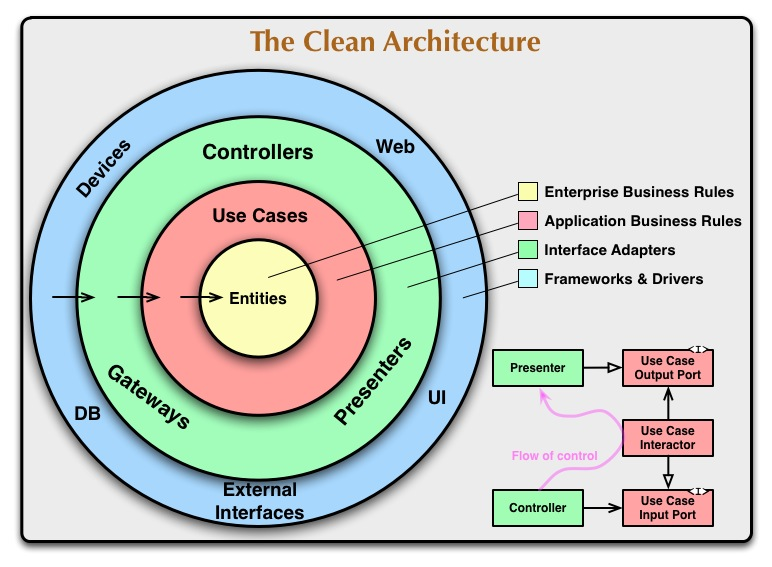
\includegraphics[width=13cm]{imgs/ch4_clean_architecture.jpg}
    \caption
{Clean architecture of Android według Uncle Ben. Źródło: \url{http://blog.8thlight.com/uncle-bob/2012/08/13/the-clean-architecture.html}}
    \label{fig:clean_architecture}
\end{figure} 

Idea tego schematu jest następująca:

\begin{itemize}

\item
Najważniejszym elementem jest środek, czyli warstwa \textit{Entities}. W warstwie tej znajdują się kluczowe dla tworzonej aplikacji reguły biznesowe gwarantujące poprawność działania programu. Krótko mówiąc – znajduje się tam logika działania aplikacji.
\item
Drugą warstwą są \textit{Use Cases}. W wolnym tłumaczeniu są to przypadki użycia, ale lepiej chyba używać nazwy intencje biznesowe. Jest to zbiór wszystkich zachowań, jakich oczekujemy od tworzonego systemu. W przypadku aplikacji bankowej, może być to na przykład funkcja wykonywania przelewu, jako jeden \textit{use case}, a innym przypadkiem użycia byłoby sprawdzenie stanu konta.
\item
Wyższa, otaczająca warstwa dotyczy wszystkich kontrolerów i prezenterów. Warto zauważyć, że nadal na tym etapie nie mamy powiązania z systemem Android.
\item
Dopiero na ostatniej, najbardziej zewnętrznej warstwie pojawia nam się powiązanie z Android SDK. Korzystamy z niego aby dostać się do baz danych, skorzystać z interfejsów użytkownika dla danego urządzenia, uzyskać dostęp do zewnętrznych interfejsów lub urządzeń.
\end{itemize}

I teraz rzecz najważniejsza: pomiędzy warstwami na schemacie narysowane są strzałki, które informują nas o kierunku przekazywania informacji. Ze schematu wynika, że \textit{Entities} nie wiedzą nic o istnieniu \textit{Use Cases}, \textit{Use Cases} nie posiadają informacji o kontrolerach i prezenterach, a te z kolei nie wiedzą o istnieniu interfejsu użytkownika. Patrząc w drugą stronę, każda warstwa wyższa posiada wszystkie informacje o warstwie niższej, czyli UI wie wszystko o prezenterach, te wiedzą wszystko o \textit{Use Cases}, no i przypadki użycia mogą korzystać z całej warstwy logicznej.

Przekładając to na język języków programowania, jeżeli używamy instrukcji \texttt{import android.*}, to tylko w stosunku do wyższej warstwy. Nie wolno nam tego robić w stosunku do warstwy niższej, bo wtedy cała koncepcja zostanie zachwiana.

W ten sposób teoretycznie jesteśmy w stanie stworzyć architekturę, która:
\begin{itemize}
\item
jest niezależna od frameworka (tutaj Android SDK) – i zachowujemy zasadę zależności,
\item
jest niezależna od UI, bazy danych lub innych urządzeń zewnętrznych,
\item
jest testowalna, w oderwaniu od warstwy zawierającej interfejsy wymienione powyżej, czyli od wszystkiego, co czyni testy na Androidzie trudnymi.
\end{itemize}

Jeżeli ułożymy naszą strukturę aplikacji w powyższy sposób – testowanie powinno odbywać się jak w przypadku kodu napisanego w czystej Javie czy C++.

\section{Praca z kodem zastanym}
\label{legacy_code}
W rozdziale \ref{pielegnowalnosc_aplikacji} nawiązaliśmy już do problemu pracy z kodem zastanym, tak zwanym \textit{Legacy Code}.
Co więc zrobić, aby zaimplementować testy do już napisanego kodu? Godfrey Nolan\footnote{Godfrey Nolan - założyciel i prezes RIIS LLC, firmy zajmującej się rozwojem oprogramowania dla platform przenośnych. Autor książek o Androidzie: "Agile Android", "Booletproof android", "Android Best Practices" i "Decompiling Android"} w swojej książce "Agile Android"\cite{bib:agile:android} proponuje następujące rozwiązanie:

\begin{itemize}
\item 
Wprowadzić metodę ciągłej integracji w procesie budowania kodu -  (\textit{Continuous Integration (CI)}).

Jest to należąca do metodologii zwinnych praktyka polegająca na regularniej integracji zmian w kodzie do bieżącego repozytorium. Warunkiem koniecznym umieszczenia kodu w repozytorium jest upewnienie się, że dany kod działa.

\item
Przy projektowaniu nowych funkcjonalności używać metody TDD.

\item
Skorzystać z serwera CI (dobrym przykładem jest tutaj \textit{Jenkins}\footnote{http://jenkins-ci.org/}), który będzie wykonywał unit testy, do których mamy przekonanie, że ich implementacja nie powinna się zmieniać. Oczywiście tylko na tym etapie, bo testy automatyczne muszą również podlegać przeglądom.

\item
Uświadomić zespół programistów na czym polegają testy jednostkowe i przekonać ich do stosowania TDD.

\item
Dodać metryki mierzenia kodu do CI. Ustawić poziom minimalny na 10-15\%.

\item
Użyć frameworka do podstawowych testów GUI już istniejącej aplikacji (najlepiej \textit{Espresso}). Stworzyć testy opierając się na przypadkach użycia (ang. \textit{use cases)}.

\item
Bezwzględnie pisać testy jednostkowe do nowych części oprogramowania zgodnie z TDD, \textit{mockując} jeśli to możliwe wykorzystywane obiekty z zastanego kodu.

\item
Wyizolować zastany kod, tak aby nikt z programistów nie miał do niego dostępu, jeżeli naprawdę nie musi.

\item
Usunąć niewykorzystywane i nieużyteczne części kodu.

\item
Przepisać i przetestować wyizolowany kod, aby zwiększyć metryki pokrycia do około 60-70\%. 
\end{itemize}

Najważniejsze więc jest wyizolować stary kod, przetestować aplikację za pomocą frameworka do testów GUI, usunąć ewentualne błędy niepozwalające na poprawną pracę programu i nie modyfikować wyizolowanego kodu podczas pisania nowych funkcjonalności. Nowe funkcje należy dodawać stosując już TDD. Dopiero na końcu, jeżeli nasze środowisko jest już stabilne, należy rozpocząć przebudowę starych części aplikacji, tak aby metryki pokrycia kodu rosły wraz z upływem czasu. Przy wykonywaniu \textit{refaktoringu} Godfrey Nolan proponuje użyć narzędzia SonarQube\footnote{SonarQube - platforma do prowadzenia ciągłej inspekcji jakości kodu źródłowego, dostarczana na licencji \textit{open source}}.